\documentclass[10pt,letterpaper,twocolumn]{article}

\usepackage[T1]{fontenc}
\usepackage{lmodern}
\usepackage[margin=0.62in,columnsep=0.27in]{geometry}
\usepackage{amsmath,amssymb,mathtools,bm}
\usepackage{array,booktabs,tabularx}
\usepackage{graphicx}
\usepackage{xcolor}
\usepackage{enumitem}
\usepackage{microtype}
\usepackage{fancyhdr}
\usepackage{hyperref}
\usepackage{needspace}

\graphicspath{{figures/}}

% The user-local tools/array package is newer than the available LaTeX kernel.
\makeatletter
\def\vcenter@text{\vbox}
\makeatother

\definecolor{navy}{HTML}{17365D}
\definecolor{blue}{HTML}{2B6CB0}
\definecolor{green}{HTML}{2F6B4F}
\definecolor{palegreen}{HTML}{EDF7F1}
\definecolor{pale}{HTML}{F3F7FB}
\definecolor{brick}{HTML}{9B2C2C}

\hypersetup{
  colorlinks=true,
  linkcolor=navy,
  urlcolor=blue,
  pdftitle={Addendum Part II: Correction Solver, Validation, and Closure Attribution},
  pdfauthor={Holstein-dimer stability calculation}
}

\pagestyle{fancy}
\fancyhf{}
\fancyhead[L]{\footnotesize Holstein-dimer stability addendum, Part II}
\fancyhead[R]{\footnotesize Correction solver and closure attribution}
\fancyfoot[C]{\thepage}
\renewcommand{\headrulewidth}{0.3pt}

\setlength{\parindent}{0pt}
\setlength{\parskip}{2.8pt plus 0.5pt}
\setlist{nosep,leftmargin=*,topsep=2pt}
\renewcommand{\arraystretch}{1.09}
\newcolumntype{Y}{>{\raggedright\arraybackslash}X}

\newcommand{\R}{\mathbb R}
\newcommand{\C}{\mathbb C}
\newcommand{\I}{\mathbb I}
\newcommand{\ii}{\mathrm i}

\newcommand{\segmenthead}[1]{%
  \Needspace{5\baselineskip}%
  \par\medskip{\color{navy}\large\bfseries #1}\par
  \vspace{-2pt}{\color{navy}\rule{\columnwidth}{0.7pt}}\par\smallskip
}
\newcommand{\conceptbreak}{%
  \par\smallskip\noindent
  {\color{black!30}\rule{\columnwidth}{0.35pt}}%
  \par\smallskip
}
\newcommand{\teachbox}[2]{%
  \par\smallskip
  \noindent\begin{minipage}{\columnwidth}
    {\color{#1}\rule{\columnwidth}{1.0pt}}\par\vspace{-1pt}
    \small\textbf{\color{#1}#2}\par\smallskip\color{black}
}
\newcommand{\closeteachbox}{%
  \par\vspace{1pt}{\color{navy!35}\rule{\columnwidth}{0.35pt}}
  \end{minipage}\par\smallskip
}

\begin{document}
\raggedbottom
\setcounter{page}{23}

\twocolumn[
\begin{center}
  {\color{navy}\LARGE\bfseries Addendum Part II}\par\vspace{3pt}
  {\Large Correction Solver, Validation, and Closure Attribution}\par\vspace{4pt}
  {\small Continuation after the printed original (pp.~1--14) and printed
  Addendum Part I (pp.~15--22), 2 August 2026}
\end{center}
\vspace{3pt}
\hrule
\vspace{7pt}
]

\textbf{Print boundary and notation amendment.}
Pages 1--22 are the fixed printed record.  This document begins at page 23
and contains the later correction and expansion.  Printed Addendum Part I
called the velocity-correction vector \(u\); Part II uses

\[
w=(w_0,\ldots,w_{30})\in\R^{31}.
\]

Both symbols denote the same controller.  The requested inward flux equals
zero, so its identity-matrix contribution vanishes.  The active barrier
parameters are \(\beta=5\) and \(h_\star=10^{-5}\).

\segmenthead{A. The correction coordinates and their lift}

The optimization chooses a correction in the 31-real-coordinate velocity
space, while the physicality conditions act on electronic and joint-Gram
matrices.  The lift connects these two representations.

At one right-hand-side evaluation, the archive equations supply the raw
coordinate velocity
\[
\dot x_0=f(t,x)\in\R^{31}.
\tag{II.1}
\]
The correction \(w\in\R^{31}\) uses the same coordinate ordering as \(x\) and
forms the corrected instantaneous velocity
\[
\dot x_{\rm c}=f(t,x)+w,
\tag{II.2}
\]
The integrator advances the current state by integrating this corrected
velocity.  Each entry of \(w=(w_0,\ldots,w_{30})\) occupies the same slot as
the corresponding entry of \(x\).  The \emph{lift} below places these 31 real
coefficients into the electronic, phononic, and correlation matrix
velocities.  Its repeated and conjugated entries preserve the Hermitian,
symmetric, and shared-trace structure built into the coordinate
representation.

The electronic-density and coherent-phonon parts are
\[
\begin{aligned}
\Delta\dot\rho(w)&=
\begin{pmatrix}
w_0/2&w_1+\ii w_2\\
w_1-\ii w_2&-w_0/2
\end{pmatrix},\\[2pt]
\Delta\dot B(w)&=
\begin{pmatrix}w_3+\ii w_4\\w_5+\ii w_6\end{pmatrix}.
\end{aligned}
\tag{II.4}
\]
The normal and anomalous phonon second moments receive
\[
\begin{aligned}
\Delta\dot N(w)&=
\begin{pmatrix}
w_7&w_9+\ii w_{10}\\
w_9-\ii w_{10}&w_8
\end{pmatrix},\\
\Delta\dot A(w)&=
\begin{pmatrix}
w_{11}+\ii w_{12}&w_{15}+\ii w_{16}\\
w_{15}+\ii w_{16}&w_{13}+\ii w_{14}
\end{pmatrix}.
\end{aligned}
\tag{II.5}
\]
Consequently the bosonic moment-matrix velocity is
\[
\Delta\dot M_{\rm B}(w)=
\begin{pmatrix}
\Delta\dot N(w)^{\mathsf T}&\Delta\dot A(w)^\ast\\
\Delta\dot A(w)&\Delta\dot N(w)
\end{pmatrix}.
\tag{II.6}
\]
The identity block in \(M_{\rm B}\) has zero derivative.

The two electron--phonon correlation matrices receive
{\scriptsize
\[
\begin{aligned}
\Delta\dot C^0(w)&=
\begin{pmatrix}
\frac{w_{17}+\ii w_{18}+w_{19}+\ii w_{20}}2&w_{21}+\ii w_{22}\\
w_{23}+\ii w_{24}&\frac{w_{17}+\ii w_{18}-w_{19}-\ii w_{20}}2
\end{pmatrix},\\[3pt]
\Delta\dot C^1(w)&=
\begin{pmatrix}
\frac{w_{17}+\ii w_{18}+w_{25}+\ii w_{26}}2&w_{27}+\ii w_{28}\\
w_{29}+\ii w_{30}&\frac{w_{17}+\ii w_{18}-w_{25}-\ii w_{26}}2
\end{pmatrix}.
\end{aligned}
\tag{II.7}
\]
}
The first two correlation coordinates are the real and imaginary parts of the
shared trace \(s=\operatorname{Tr}C^q\).

The joint electron--phonon Gram matrix has the block form
\[
\mathcal G=
\begin{pmatrix}
M_{\rm B}(N,A)&Z(C)\\
Z(C)^\dagger&E(\rho)
\end{pmatrix},
\tag{II.8}
\]
where \(M_{\rm B}\) is the bosonic moment block, \(Z(C)\) is the
electron--phonon cross-Gram block, and \(E(\rho)\) is the electronic Gram
block.  Differentiating these three block constructions along the lifted
velocity gives
\[
\Delta\dot{\mathcal G}(w)=
\begin{pmatrix}
\Delta\dot M_{\rm B}(w)&\Delta\dot Z(w)\\
\Delta\dot Z(w)^\dagger&\Delta\dot E(w)
\end{pmatrix}.
\tag{II.9}
\]
Thus a 31-real-coordinate vector changes a \(7\times7\) Hermitian matrix
velocity while retaining the same 31 independent degrees of freedom.

\segmenthead{B. The differential barriers and the constrained problem}

Let \(m(t)\) denote one eigenvalue margin measured from a PSD boundary.  The
positive number \(h_\star\) is the desired safety margin, and \(\beta>0\) is
the rate at which a smaller margin must recover.  The scalar differential
barrier is
\[
\dot m+\beta(m-h_\star)\geq0.
\tag{II.10}
\]
Multiplication by the integrating factor \(e^{\beta t}\) gives
\[
\frac{d}{dt}\!\left[e^{\beta t}(m-h_\star)\right]\geq0,
\]
and integration from \(0\) to \(t\) gives
\[
m(t)\geq h_\star+[m(0)-h_\star]e^{-\beta t}.
\tag{II.11}
\]
At \(m=h_\star\), the condition requires \(\dot m\geq0\).  For
\(m>h_\star\), the available margin determines the permitted outward rate.
The requested additional inward flux is zero.

The matrix barrier applies the same condition simultaneously to every
eigenvalue direction.  Reconstruct the raw matrix velocities
\(\dot\rho_0\) and \(\dot{\mathcal G}_0\) from
\(\dot x_0=f(t,x)\).  Let \(I_2\) and \(I_7\) be the identity matrices in the
electronic and joint-Gram spaces.  The three raw differential-barrier matrices
and their correction responses are
{\footnotesize
\[
\begin{aligned}
M_{0,\rho^-}
&=\dot\rho_0+\beta(\rho-h_\star I_2),
&\Delta M_{\rho^-}(w)&=\Delta\dot\rho(w),\\
M_{0,\rho^+}
&=-\dot\rho_0+\beta(I_2-\rho-h_\star I_2),
&\Delta M_{\rho^+}(w)&=-\Delta\dot\rho(w),\\
M_{0,\mathcal G}
&=\dot{\mathcal G}_0+\beta(\mathcal G-h_\star I_7),
&\Delta M_{\mathcal G}(w)&=\Delta\dot{\mathcal G}(w).
\end{aligned}
\tag{II.12}
\]
}
Each Hermitian matrix in (II.12) evaluates one differential barrier under the
raw archive velocity; the subscript \(0\) identifies this raw evaluation.  A
negative eigenvalue identifies a matrix direction whose margin evolves faster
than the barrier permits.  The expression in the adjacent right-hand column
is the matrix change produced when \(w\) is added to the coordinate velocity.

The trace variable and energy functional complete the constraints.  Define
\[
s=\operatorname{Tr}C^0=\operatorname{Tr}C^1
=x_{17}+\ii x_{18},
\qquad
\dot s_0=\dot x_{0,17}+\ii\dot x_{0,18},
\]
and let \(E_{\rm int}(x)\) be the internal energy with coordinate gradient
\(\nabla_xE_{\rm int}(x)\in\R^{31}\).  The implemented correction is the
minimum-Euclidean-norm feasible velocity:
{\footnotesize
\[
\begin{aligned}
\underset{w\in\R^{31}}{\operatorname{minimize}}\quad
&\tfrac12\lVert w\rVert_2^2\\
\text{subject to}\quad
&M_{0,\rho^-}+\Delta M_{\rho^-}(w)\succeq0,\\
&M_{0,\rho^+}+\Delta M_{\rho^+}(w)\succeq0,\\
&M_{0,\mathcal G}+\Delta M_{\mathcal G}(w)\succeq0,\\
&\dot s_0+w_{17}+\ii w_{18}+\beta s=0,\\
&\nabla_xE_{\rm int}(x)^{\mathsf T}w=0.
\end{aligned}
\tag{II.13}
\]
}
The first two inequalities protect the lower and upper eigenvalue boundaries
of the one-body electronic density.  The third protects the joint
electron--phonon Gram matrix.  The complex trace line is two real equalities;
it implies
\[
\dot s_{\rm c}=-\beta s,
\qquad s(t)=s(0)e^{-\beta t}.
\tag{II.14}
\]
The final equality makes the \emph{added} velocity energy-neutral:
\[
\frac{dE_{\rm int}}{dt}
=\nabla_xE_{\rm int}^{\mathsf T}f(t,x)
+\underbrace{\nabla_xE_{\rm int}^{\mathsf T}w}_{=0}.
\tag{II.15}
\]
Thus the corrected and raw velocities have the same instantaneous
internal-energy change; the time-dependent drive retains its physical work.

\segmenthead{C. From the constrained velocity to the minimum correction}

At one Runge--Kutta evaluation point \((t,x)\), the archive equations give
the raw velocity \(\dot x_0=f(t,x)\in\R^{31}\).  The correction
\(w\in\R^{31}\) forms \(\dot x_{\rm c}=\dot x_0+w\).  The equality rows are
\(Lw=d\), and one of the three corrected differential-barrier matrices will
be denoted simply by \(M(w)\).  The same derivation is applied to the lower
electronic barrier, the upper electronic barrier, and the joint-Gram barrier.
The local problem is
\[
\begin{aligned}
w^\star\in\underset{w\in\R^{31}}{\operatorname{argmin}}\quad
&\tfrac12\lVert w\rVert_2^2\\
\text{subject to}\quad
&Lw=d,\\
&M(w)\succeq0
\quad\text{for all three barrier matrices}.
\end{aligned}
\tag{II.16}
\]
The solution proceeds in a fixed order.  The energy and trace equations first
determine the part of \(w\) required by those three scalar equalities.  The
remaining directions preserve those equalities and are therefore available
to repair the three matrix inequalities.  This separation turns the full
problem into the shortest correction inside the intersection of the allowed
matrix half-spaces.

Coordinates \(x_{17}\) and \(x_{18}\) store the real and imaginary parts of
the shared correlation trace \(s=x_{17}+\ii x_{18}\).  Define the linear map
\(L:\R^{31}\to\R^3\) by letting its first output be the correction-induced
energy flux and its next two outputs be the correction to the real and
imaginary trace velocities:
{\footnotesize
\[
Lw=
\begin{pmatrix}
\nabla_xE_{\rm int}(x)^{\mathsf T}w\\
w_{17}\\
w_{18}
\end{pmatrix}
,qquad
d=
\begin{pmatrix}
0\\
-\dot x_{0,17}-\beta x_{17}\\
-\dot x_{0,18}-\beta x_{18}
\end{pmatrix}
\in\R^3.
\tag{II.17}
\]
}
The equality condition is \(Lw=d\); as a matrix,
\(L\in\R^{3\times31}\).  Let \(r=\operatorname{rank}L\).  Its reduced singular-value
decomposition is
\[
L=U_r\Sigma_rV_r^{\mathsf T},
\tag{II.18}
\]
where the columns of \(U_r\in\R^{3\times r}\) and
\(V_r\in\R^{31\times r}\) are orthonormal, while
\(\Sigma_r\in\R^{r\times r}\) is diagonal with positive singular values.
This factorization writes the map \(w\mapsto Lw\) as the consecutive chain
\[
w\ \longmapsto\ V_r^{\mathsf T}w
\ \longmapsto\ \Sigma_rV_r^{\mathsf T}w
\ \longmapsto\ U_r\Sigma_rV_r^{\mathsf T}w=Lw.
\tag{II.18a}
\]
The first arrow measures how much of \(w\) lies along each correction
direction that affects the equalities.  The diagonal matrix \(\Sigma_r\)
scales those measured components by their strength, and \(U_r\) combines the
scaled components into the energy row and the two trace rows.  The columns of
\(V_r\) therefore span every correction direction visible to \(L\).

Complete these visible directions with an orthonormal matrix
\(Q\in\R^{31\times(31-r)}\) satisfying
\[
V_r^{\mathsf T}Q=0,
\qquad
Q^{\mathsf T}Q=I_{31-r},
\qquad
LQ=U_r\Sigma_rV_r^{\mathsf T}Q=0.
\tag{II.19}
\]
The columns of \(Q\) span the remaining correction directions.  Since
\(LQ=0\), motion along any combination of these columns changes none of the
three constrained scalars.  Every correction has the unique decomposition
\[
w=V_r\alpha+Qy,
\qquad
\alpha\in\R^r,\quad y\in\R^{31-r}.
\tag{II.20}
\]
Here \(\alpha\) measures the equality-changing part and \(y\) measures the
equality-preserving part.  Substitution into \(Lw=d\) determines \(\alpha\):
\[
\begin{aligned}
Lw
&=U_r\Sigma_rV_r^{\mathsf T}(V_r\alpha+Qy)\\
&=U_r\Sigma_r\alpha=d,\\
\alpha&=\Sigma_r^{-1}U_r^{\mathsf T}d.
\end{aligned}
\tag{II.20a}
\]
The equality-fixed part of the correction is therefore
\[
w_{\rm p}
=V_r\Sigma_r^{-1}U_r^{\mathsf T}d
=L^+d,
\qquad
w=w_{\rm p}+Qy,
\tag{II.20b}
\]
where \(L^+=V_r\Sigma_r^{-1}U_r^{\mathsf T}\) is the Moore--Penrose
pseudoinverse on the nonzero singular directions.  Orthogonality gives
\[
\lVert w\rVert_2^2
=\lVert w_{\rm p}\rVert_2^2+
\lVert Qy\rVert_2^2
=\lVert w_{\rm p}\rVert_2^2+
\lVert y\rVert_2^2.
\tag{II.21}
\]
The equality rows fix \(w_{\rm p}\).  The PSD constraints choose the shortest
remaining coordinate \(y\).  The rest of the derivation therefore works
entirely within this equality-preserving space.

Choose one of the three raw barrier matrices and call it \(M_0\).  Its
correction lift is \(\Delta M(w)\), and the corrected Hermitian matrix is
\[
M(w)=M_0+\Delta M(w)\in\C_{\rm H}^{m\times m},
\qquad m=2\ \text{or}\ 7.
\tag{II.22}
\]
For the lower electronic barrier,
\(M_0=\dot\rho_0+\beta(\rho-h_\star I_2)\) and
\(\Delta M(w)=\Delta\dot\rho(w)\).  For the upper electronic barrier, the
pair is \(-\dot\rho_0+\beta(I_2-\rho-h_\star I_2)\) and
\(-\Delta\dot\rho(w)\).  For the joint barrier, the pair is
\(\dot{\mathcal G}_0+\beta(\mathcal G-h_\star I_7)\) and
\(\Delta\dot{\mathcal G}(w)\).

Let \(k\) index the cutting-plane iterations.  At the current reduced
coordinate \(y^{(k)}\), reconstruct
\(w^{(k)}=w_{\rm p}+Qy^{(k)}\) and diagonalize \(M(w^{(k)})\).  Let
\(\lambda<0\) be its minimum eigenvalue and let \(v\in\C^m\) be the
corresponding normalized eigenvector:
\[
M(w^{(k)})v=\lambda v,
\qquad v^\dagger v=1,
\qquad \lambda=\lambda_{\min}(M(w^{(k)}))<0.
\tag{II.23}
\]
The vector \(v=(v_1,\ldots,v_m)^{\mathsf T}\) contains the coefficients of
the particular linear combination of matrix rows and columns that currently
has the smallest margin.  It lives in the \(m\)-dimensional matrix space,
whereas \(w\) lives in the 31-dimensional coordinate-velocity space.  The
quadratic form \(v^\dagger Mv\) evaluates the matrix margin for this normalized
combination: multiply \(M\) by \(v\), then take its complex inner product with
\(v\).  For the eigenvector in (II.23), this scalar is
\[
v^\dagger M(w^{(k)})v
=v^\dagger(\lambda v)
=\lambda.
\tag{II.23a}
\]
The required inequality must now be written in the 31 scalar coordinates of
\(w\).  A linear map is determined by its response to each unit coordinate
direction.  Define
\[
e_j=(0,\ldots,0,\underbrace{1}_{j\text{th slot}},0,\ldots,0)^{\mathsf T}
\in\R^{31},
\qquad j=0,\ldots,30.
\tag{II.24}
\]
The vector \(e_j\) activates one correction coefficient.  Its lift
\(\Delta M(e_j)\) is the complete Hermitian matrix pattern produced by one
unit of \(w_j\).  This is why \(e_j\) is introduced here: it lets us measure,
one coordinate at a time, how the 31-component correction changes the
currently failing matrix combination.  Therefore
\[
\begin{aligned}
w-w^{(k)}
&=\sum_{j=0}^{30}(w_j-w_j^{(k)})e_j,\\
\Delta M(w-w^{(k)})
&=\sum_{j=0}^{30}(w_j-w_j^{(k)})\Delta M(e_j).
\end{aligned}
\tag{II.24a}
\]
Contract each lifted pattern along the failing eigenvector and define its real
sensitivity
\[
\begin{aligned}
a_j
&=v^\dagger\Delta M(e_j)v\\
&=\sum_{r=1}^{m}\sum_{s=1}^{m}
v_r^*[\Delta M(e_j)]_{rs}v_s\in\R,
\end{aligned}
\qquad
a=(a_0,\ldots,a_{30})\in\R^{31}.
\tag{II.24b}
\]
The number \(a_j\) is the change in the exposed scalar barrier per unit change
of \(w_j\).  The complete vector \(a\) translates a coordinate correction
into a change of the failing scalar margin.  Linearity now produces the
complete chain
\[
\begin{aligned}
v^\dagger M(w)v
&=v^\dagger\!\left[
M(w^{(k)})+\Delta M(w-w^{(k)})
\right]v\\
&=\lambda+
\sum_{j=0}^{30}a_j(w_j-w_j^{(k)})\\
&=\lambda+a^{\mathsf T}(w-w^{(k)}).
\end{aligned}
\tag{II.25}
\]
Requiring this scalar to be nonnegative gives the half-space
\[
a^{\mathsf T}w
\geq a^{\mathsf T}w^{(k)}-\lambda.
\tag{II.25a}
\]
The vector \(a\) is normal to the half-space boundary.  A feasible correction
produces a lifted matrix change whose value along \(v\) supplies the missing
positive amount \(-\lambda\).

The equality-preserving coordinates now convert this matrix requirement into
the actual minimum problem.  Substitute
\(w=w_{\rm p}+Qy\) and \(w^{(k)}=w_{\rm p}+Qy^{(k)}\) into the half-space.
The fixed particular correction cancels:
\[
\begin{aligned}
a^{\mathsf T}(w_{\rm p}+Qy)
&\geq a^{\mathsf T}(w_{\rm p}+Qy^{(k)})-\lambda,\\
(Q^{\mathsf T}a)^{\mathsf T}y
&\geq (Q^{\mathsf T}a)^{\mathsf T}y^{(k)}-\lambda.
\end{aligned}
\]
Define
\[
n=Q^{\mathsf T}a,
\qquad
c=n^{\mathsf T}y^{(k)}-\lambda.
\tag{II.26}
\]
The vector \(n\in\R^{31-r}\) is the half-space normal expressed in the free
SVD coordinates, and \(c\in\R\) is the amount that their overlap must reach.
For one cut, the equality-reduced problem is
\[
\begin{aligned}
\underset{y\in\R^{31-r}}{\operatorname{minimize}}\quad
&\tfrac12y^{\mathsf T}y\\
\text{subject to}\quad&n^{\mathsf T}y\geq c.
\end{aligned}
\tag{II.26a}
\]
Introduce the nonnegative optimization multiplier \(\mu\).  When \(c>0\),
the shortest feasible vector reaches the half-space boundary.  The
Karush--Kuhn--Tucker conditions then give
\[
\begin{aligned}
\mathcal L(y,\mu)
&=\tfrac12y^{\mathsf T}y-\mu(n^{\mathsf T}y-c),\\
\nabla_y\mathcal L=y-\mu n&=0,\\
n^{\mathsf T}y-c&=0,\\
y^\star&=\frac{c}{\lVert n\rVert_2^2}\,n,
\qquad
w^\star=w_{\rm p}+Qy^\star.
\end{aligned}
\tag{II.27}
\]
When \(c\leq0\), the origin \(y=0\) already satisfies the cut and is the
shortest choice.  Thus one cut either leaves the equality-only correction
\(w_{\rm p}\) unchanged or adds the shortest free-space displacement parallel
to \(n\).
This is the shortest equality-feasible correction for one exposed matrix
direction.  With no equality rows, \(Q=I_{31}\), \(w_{\rm p}=0\),
\(n=a\), and the first negative cut has \(c=-\lambda\); the formula becomes
\[
w^\star=\frac{-\lambda}{\lVert a\rVert_2^2}\,a,
\qquad
v^\dagger M(w^\star)v
=\lambda+a^{\mathsf T}w^\star=0.
\tag{II.27a}
\]

For the complete matrix, positive semidefiniteness requires the quadratic form
to be nonnegative in every normalized matrix direction:
\[
M(w)\succeq0
\quad\Longleftrightarrow\quad
\xi^\dagger M(w)\xi\geq0
\ \text{for every }\xi^\dagger\xi=1,
\qquad
\lambda_{\min}(M(w))
=\min_{\xi^\dagger\xi=1}\xi^\dagger M(w)\xi.
\tag{II.28}
\]
The current cut controls the exposed direction \(\xi=v\).  Rebuilding the
complete matrix identifies the direction that now attains the minimum.  After
\(p\) exposed directions, let \(n_i,c_i\) be the normal and offset of cut
\(i\).  The accumulated solve is
\[
\begin{aligned}
\underset{y\in\R^{31-r}}{\operatorname{minimize}}\quad
&\tfrac12y^{\mathsf T}y\\
\text{subject to}\quad
&n_i^{\mathsf T}y\geq c_i,
\qquad i=1,\ldots,p.
\end{aligned}
\tag{II.28a}
\]
SLSQP computes the shortest \(y\) in the intersection of these half-spaces.
The program reconstructs \(w=w_{\rm p}+Qy\), rebuilds all three complete
barrier matrices, diagonalizes them, and adds the next failing direction.  The
cycle terminates when every eigenvalue reaches the declared tolerance.  Near a
degenerate minimum, the fallback asks SLSQP to enforce every eigenvalue of all
three matrices directly.  At the exact cutoff-16 initial state, the
cutting-plane and direct spectral solutions agreed in correction norm to
relative tolerance \(2\times10^{-7}\).

\conceptbreak
\textbf{Which norm was minimized.}
The implemented objective is
\[
\tfrac12\lVert w\rVert_2^2
=\tfrac12\sum_{j=0}^{30}w_j^2.
\tag{II.29}
\]
It minimizes the independent real coordinate coefficients in the displayed
31-coordinate scaling.  The Frobenius size of the lifted matrix entries has
the form
\[
\begin{aligned}
&\lVert\Delta\dot\rho\rVert_{\rm F}^2
+\lVert\Delta\dot B\rVert_2^2
+\lVert\Delta\dot N\rVert_{\rm F}^2
+\lVert\Delta\dot A\rVert_{\rm F}^2\\
&\qquad+\sum_q\lVert\Delta\dot C^q\rVert_{\rm F}^2
=w^{\mathsf T}Ww,
\qquad W\neq I_{31}.
\end{aligned}
\tag{II.30}
\]
Repeated conjugate entries, symmetric copies, and one-half factors create the
weights in \(W\).  Therefore the implemented correction is coordinate-
Euclidean-minimum; a matrix-Frobenius-minimum controller would use
\(w^{\mathsf T}Ww/2\).

\segmenthead{D. How the correction enters RK4}

Define the corrected right-hand side
\[
f_{\rm c}(t,x)=f(t,x)+w^\star(t,x),
\tag{II.31}
\]
where \(w^\star(t,x)\) is obtained by reconstructing the matrices at that
specific time and state and minimizing its Euclidean norm subject to the
electronic, joint-Gram, correlation-trace, and energy conditions.  One fixed
RK4 step is
{\footnotesize
\[
\begin{aligned}
k_1&=f_{\rm c}(t_n,x_n),\\
k_2&=f_{\rm c}(t_n+h/2,x_n+hk_1/2),\\
k_3&=f_{\rm c}(t_n+h/2,x_n+hk_2/2),\\
k_4&=f_{\rm c}(t_n+h,x_n+hk_3),\\
x_{n+1}&=x_n+\frac h6(k_1+2k_2+2k_3+k_4).
\end{aligned}
\tag{II.32}
\]
}
Each \(k_i\in\R^{31}\) is a corrected instantaneous velocity.  Multiplying
by \(h\) turns that rate into a coordinate increment.  The provisional states
inside \(k_2,k_3,k_4\) are different, so every occurrence of \(f_{\rm c}\)
performs a fresh matrix reconstruction and a fresh constrained solve.
The four stage evaluations are solver-internal.  The accepted \(x_{n+1}\) is
the stored or plotted trajectory sample.

For \(h=0.01\), the \(t=1000\) trajectory contains 100,000 stored steps and
400,000 corrected right-hand-side evaluations.  The correction enters each
stage velocity \(k_i\), and the weighted stage sum produces \(x_{n+1}\).

\newpage
\segmenthead{E. How the implementation and result were checked}

\begin{center}
\small
\begin{tabularx}{\columnwidth}{@{}Y Y@{}}
\toprule
check & what it establishes\\
\midrule
100 random 13-coordinate derivative comparisons, tolerance
\(2\times10^{-15}\) & the handwritten scalar and reconstructed archive
matrix routes assign the same shared derivatives\\
100 coordinate round trips and matrix-tangency checks & extraction and
reconstruction preserve the 31-coordinate state; generated velocities remain
inside its represented structural subspace\\
centered finite differences of the lift and energy functional, tolerance
\(10^{-8}\) & the analytic matrix lift and energy covector give the measured
first-order changes\\
cutting-plane versus direct spectral solve & both optimizers reach the same
tested correction norm and satisfy the complete constraints\\
short raw/corrected first-exit propagation & the correction changes the
predicted cone exit rather than merely relabeling a diagnostic\\
RK4 step refinement & the reported effect is larger than the measured
time-discretization change\\
exact Hamiltonian and cutoff comparisons & remaining trajectory error belongs
to the approximate closure rather than the coordinate map or cutoff-16 floor\\
\bottomrule
\end{tabularx}
\end{center}

At the exact cutoff-16 initial contractions, the raw joint barrier was below
\(-2\times10^{-3}\).  The corrected joint barrier was above \(-10^{-9}\),
the correlation-trace velocity was below \(10^{-12}\), and the added energy
flux was below \(2\times10^{-11}\).  At the recorded \(t=28.57\) state, a
restricted correction problem was infeasible while the full 31-coordinate
problem satisfied all three barriers and used nonzero correlation controls.

The raw short trajectory fell below a joint margin of \(-10^{-3}\) by
\(t=0.2\); the corrected route stayed above \(10^{-5}\), with both
correlation traces zero to \(2\times10^{-12}\).  Refining \(h=0.01\) to
\(0.005\) changed the state at \(t=2\) by \(1.18\times10^{-6}\) in
coordinate norm.

The corrected \(t=1000\) run gave
{\footnotesize
\[
\begin{aligned}
\min_t\lambda_{\min}(\mathcal G(t))&=2.06367\times10^{-5},\\
\min_t\lambda_{\min}(M_{\rm B}(t))&=2.06469\times10^{-5},\\
0.0239455\leq\lambda_{\min}(\rho(t))
&\leq\lambda_{\max}(\rho(t))\leq0.976055,\\
\max_{t,j}|x_j(t)|&=2.09860,\\
\max_{t,q}|\operatorname{Tr}C^q(t)|&=8.78\times10^{-17}.
\end{aligned}
\tag{II.33}
\]
}
Every correction solve converged.  The largest correction norm was
0.345567.  The post-pulse drift was defined by
\[
\Delta E_{\rm post}
=\max_{4\leq t\leq1000}
|E_{\rm int}(t)-E_{\rm int}(4)|
=5.03\times10^{-6}.
\tag{II.34}
\]
The reference time \(t=4\) is the declared end of the driven window: the
Gaussian pulse envelope is already negligible there and its sine factor is
zero.  This statistic asks whether internal energy subsequently drifts after
the pulse.  The maximum absolute correction-energy flux was
\(2.64\times10^{-16}\).

\teachbox{green}{What these checks do and do not prove}
They establish the coordinate transcription, the structured lift, the tested
minimum-norm constrained solve, numerical step stability, and preservation of
the selected necessary matrix conditions over the reported horizon.  They do
not establish that the 31-moment closure follows the exact Hamiltonian
dynamics.  That is a separate accuracy question.
\closeteachbox

\segmenthead{F. The offline exact-reference diagnostic}

The exact reference used the same initial state, drive, and cutoff-16
Holstein-dimer Hamiltonian.  It propagated the full truncated wavefunction by
solving
\[
\ii\frac{d}{dt}|\psi_{\rm ex}(t)\rangle
=H(t)|\psi_{\rm ex}(t)\rangle
\tag{II.35}
\]
with DOP853, an adaptive explicit eighth-order Runge--Kutta integrator.  This
was numerical integration of the time-dependent Schr\"odinger equation, not
one fixed matrix exponential.  At each saved time,
\[
|\psi_{\rm ex}(t)\rangle
\longrightarrow X_{\rm ex}(t),
\qquad
\dot X_{\rm ex}(t)=\ii\langle[H,\widehat X]\rangle_t.
\tag{II.36}
\]
The commutator supplies the exact contracted derivative at that state without
finite-differencing neighboring saved samples.

The retained correlation is the pair
\[
C=(C^0,C^1),
\qquad C^q\in\C^{2\times2},
\tag{II.37}
\]
one matrix for each phonon mode.  The symbol \(\dot C_{31}\) means the
\(C\)-block of the uncorrected 31-coordinate archive velocity.  On an exact
contracted state it is evaluated as
\[
\dot C_{31}(t)=F_C\bigl(t,X_{\rm ex}(t)\bigr),
\tag{II.38}
\]
with component form
\[
\dot C_{31}^{\,q}
=-\ii\bigl(h(t)C^q-C^qh(t)+\omega_qC^q\bigr)
+\sum_{a=0}^{4}S_a^q.
\tag{II.39}
\]
The first terms transport the existing correlation; the five archive sources
\(S_a^q\) create and modify it using the retained matrices \(\rho,N,A\).
The comparison uses the same \(X_{\rm ex}(t)\) on both sides:
\[
\dot C_{31}(t)
\quad\hbox{versus}\quad
\dot C_{\rm ex}(t)=\ii\langle[H,\widehat C]\rangle_t.
\tag{II.40}
\]
Thus it isolates a local derivative-formula error before two propagated
trajectories have separated.

Let
\[
O_{ij}=c_{j\uparrow}^\dagger c_{i\uparrow},
\quad n_{r\uparrow}=c_{r\uparrow}^\dagger c_{r\uparrow},
\quad \delta X_r=\delta b_r+\delta b_r^\dagger.
\]
The exact equation requests
\[
Q^{qr}_{ij}
=\left\langle[O_{ij},n_{r\uparrow}]\,\delta X_r\,\delta b_q\right\rangle,
\tag{II.41}
\]
whereas the second-order closure keeps the product
\[
Q^{qr}_{ij,0}
=\left\langle[O_{ij},n_{r\uparrow}]\right\rangle
 \left\langle\delta X_r\delta b_q\right\rangle.
\tag{II.42}
\]
Their connected remainder is
\[
K^{qr}_{ij}=Q^{qr}_{ij}-Q^{qr}_{ij,0}.
\tag{II.43}
\]
The two electronic covariances at the same operator line are
{\footnotesize
\[
\begin{aligned}
P^q_{ij}
&=\operatorname{Cov}(O_{ij},n_{q\uparrow})
=\delta_{iq}\rho_{qj}-\rho_{ij}\rho_{qq},\\
D^q_{ij}
&=\operatorname{Cov}(O_{ij},n_{q\downarrow})\\
&=\langle O_{ij}n_{q\downarrow}\rangle
-\rho_{ij}\langle n_{q\downarrow}\rangle.
\end{aligned}
\tag{II.44}
\]
}
Here \(P\) is fixed algebraically by the one-up-electron sector; \(D\) carries
opposite-spin information absent from the 31 retained coordinates.

Their supplied velocity terms are
\[
\boxed{
\Delta\dot C^q_{K,ij}
=-\ii g\sum_{r=0}^{1}K^{qr}_{ij},}
\tag{II.45}
\]
{\footnotesize
\[
\boxed{
\Delta\dot C^q_{P,ij}
=-\ii gP^q_{ij}
-\left[
\left(\sum_{a=0}^{4}S_a^q\right)_{ij}
+\ii g\sum_rQ^{qr}_{ij,0}
\right],}
\tag{II.46}
\]
}
and
\[
\boxed{\Delta\dot C^q_{D,ij}=-\ii gD^q_{ij}.}
\tag{II.47}
\]
The Pauli term replaces the archive's effective same-spin contribution rather
than simply adding a duplicate source.  The exact local decomposition is
\[
\boxed{
\dot C_{\rm ex}
=\dot C_{31}
+\Delta\dot C_K
+\Delta\dot C_P
+\Delta\dot C_D
+R_{\rm cut}.}
\tag{II.48}
\]

Let \(\mathcal R_C\) extract the fourteen independent real coordinates of
\(C=(C^0,C^1)\).  For supplied terms
\(S\subseteq\{K,P,D\}\), the diagnostic used
{\scriptsize
\[
\begin{aligned}
e_S(t)=\mathcal R_C\Bigl(&
 \dot C_{31}(t)+\sum_{\alpha\in S}\Delta\dot C_\alpha(t)
 -\dot C_{\rm ex}(t)\\
&-\dot C_{31}(0)-\sum_{\alpha\in S}\Delta\dot C_\alpha(0)
 +\dot C_{\rm ex}(0)\Bigr).
\end{aligned}
\tag{II.49}
\]
}
The second line removes the constant initial residual.  Over
\(0\leq t\leq4\), the sequential errors were
\[
\begin{array}{@{}lrr@{}}
\toprule
S&\operatorname{RMS}\lVert e_S\rVert_2
&\max_t\lVert e_S\rVert_2\\
\midrule
\varnothing&0.166690&0.274310\\
K&0.089345&0.137864\\
K+P&0.026160&0.038268\\
K+P+D&2.53\times10^{-5}&3.47\times10^{-5}\\
\bottomrule
\end{array}
\tag{II.50}
\]

\begin{center}
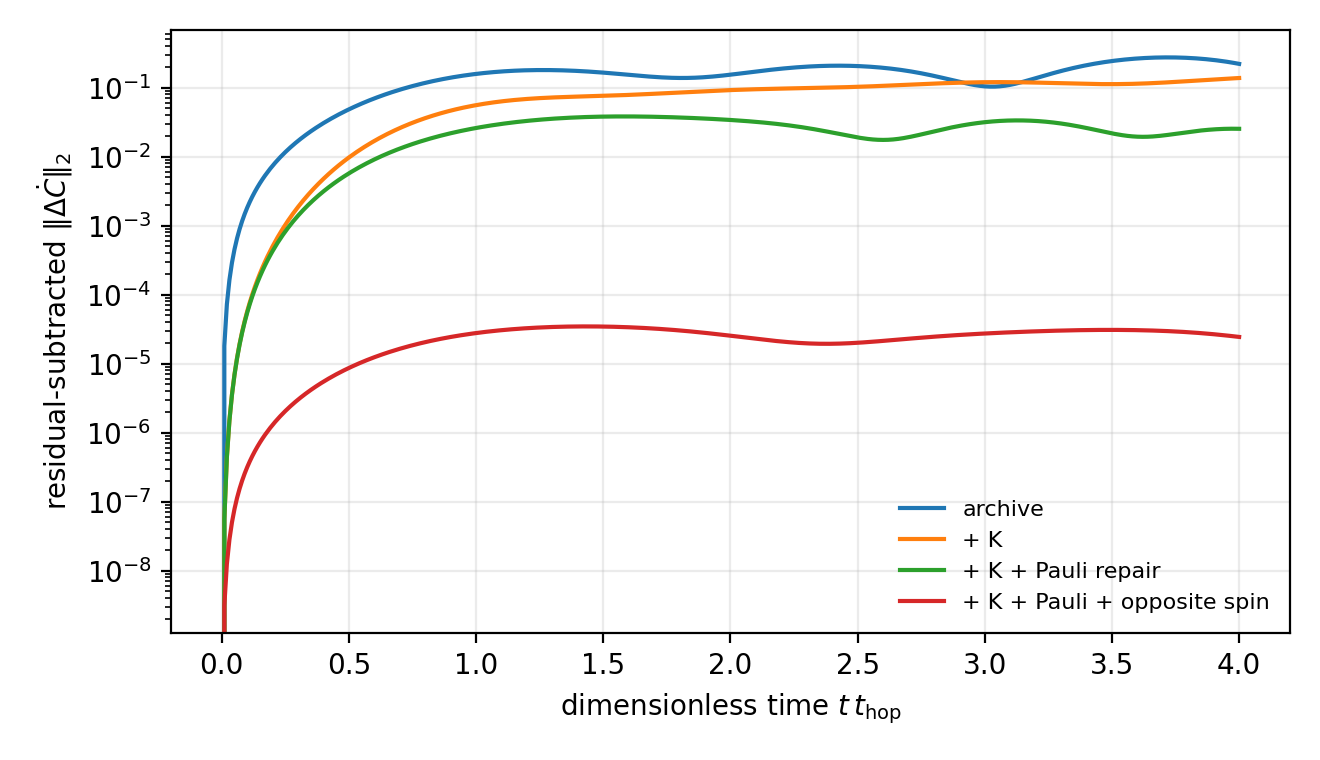
\includegraphics[width=\columnwidth]{exact_mixed_moment_closure_attribution.png}

\parbox{0.96\columnwidth}{\scriptsize
\textbf{Offline reconstruction of the missing correlation velocity.}
Every curve evaluates the archive derivative on the exact cutoff-16
trajectory.  Orange supplies \(K\), green then supplies \(P\), and red finally
supplies \(D\).  The red curve reaches the finite-cutoff remainder scale.}
\end{center}

\teachbox{brick}{Offline attribution is separate from the controller}
The exact wavefunction supplied \(K,P,D\) only for this diagnostic.  These
terms were not inserted into RK4 and were not inputs to the minimum-norm
representability correction \(w\).  The controller keeps the approximate
moments inside selected necessary matrix constraints; the \(K,P,D\) audit
identifies missing dynamics that a future autonomous closure must generate
from its own enlarged state.
\closeteachbox

\segmenthead{G. Final interpretation}

The long corrected run establishes that the joint 31-coordinate barrier can
keep the archive closure inside the retained electron--phonon moment
constraints through \(t=1000\).  The exact comparison separately establishes
that this admissible trajectory still has a converged strong-coupling accuracy
error concentrated in \(C\).  The correction stabilizes representability; it
does not repair the inaccurate moment closure.

The operator audit reconstructs the missing local \(C\)-velocity from the
connected mixed moment \(K\), the Pauli-algebra repair \(P\), and the
opposite-spin covariance \(D\), down to the finite-cutoff floor.  The next
physics task is therefore an autonomous, symmetry-adapted higher-moment
closure that evolves the required information without consulting exact
trajectory data.  The joint Gram barrier remains a separate safeguard for
that enlarged raw velocity.

\teachbox{green}{Advisor-facing summary}
I reproduced the reported strong-coupling instability, then diagnosed its
earlier physical precursor as loss of positive semidefiniteness of a retained
moment matrix.  I stabilized the selected electronic and joint
electron--phonon constraints by adding the minimum-Euclidean-norm
31-coordinate velocity correction at every RK4 stage.  Exact
truncated-Hamiltonian contractions then showed that representability was
restored but the closure remained inaccurate in the electron--phonon
correlation sector.  An offline operator audit attributed that missing local
velocity to \(K\), \(P\), and \(D\) to the cutoff floor.
\closeteachbox

\segmenthead{Questions for later oral review}

\begin{enumerate}
  \item Starting from \(x_n\), explain how the four corrected RK4 velocities
  \(k_1,\ldots,k_4\) approximate the integral that produces \(x_{n+1}\).
  \item Starting from one correction coefficient \(w_j\), trace its lift into
  \(\Delta\dot\rho\), \(\Delta\dot N\), \(\Delta\dot A\),
  \(\Delta\dot C\), and finally a barrier matrix.
  \item For one negative barrier eigenpair, distinguish \(v\), \(\lambda\),
  \(a_j\), and \(w_j\) physically and geometrically.
  \item Explain why one half-space repairs one exposed eigenvector but does
  not certify the full matrix, and then reconstruct the cutting-plane cycle.
  \item Explain why \(\lVert w\rVert_2\) and the lifted Frobenius norm use
  different metrics.
  \item Reconstruct the offline chain
  \[
  |\psi_{\rm ex}\rangle\to X_{\rm ex}
  \to\dot C_{31}\to +K\to+P\to+D
  \to\dot C_{\rm ex},
  \]
  and state why this chain was evidence, not an online correction.
\end{enumerate}

\end{document}
